\documentclass[11pt,a4paper]{article}

% =================================================================
%  Question Bank -- Unit V: Automation in Marine Industry
%  Self-contained: all block diagrams / flowcharts drawn with TikZ.
% =================================================================

\usepackage[margin=2cm, headheight=14pt]{geometry}
\usepackage{amsmath}
\usepackage{amssymb}
\usepackage{bm}
\usepackage{array}
\usepackage{booktabs}
\usepackage{enumitem}
\usepackage{xcolor}
\usepackage{tikz}
\usepackage[most]{tcolorbox}
\usepackage{fancyhdr}
\usepackage{helvet}
\renewcommand{\familydefault}{\sfdefault}
\setlength{\emergencystretch}{2em}

\usetikzlibrary{shapes.geometric, arrows.meta, positioning, calc, fit, backgrounds, patterns}

% -------------------------------------------------
% Colour palette (same as the lecture decks)
% -------------------------------------------------
\definecolor{cAccent}{RGB}{0,102,153}
\definecolor{cGreen}{RGB}{34,139,34}
\definecolor{cRed}{RGB}{178,34,34}
\definecolor{cOrange}{RGB}{204,102,0}
\definecolor{cPurple}{RGB}{102,45,145}
\definecolor{cGrayBg}{RGB}{245,246,248}

% -------------------------------------------------
% TikZ styles
% -------------------------------------------------
\tikzset{
	process/.style  ={rectangle, minimum width=2.6cm, minimum height=0.8cm, text centered, align=center, text width=2.6cm, draw=black, fill=blue!8},
	decision/.style ={diamond, aspect=2, minimum width=2.4cm, minimum height=0.9cm, text centered, text width=2.4cm, draw=black, fill=cGreen!18, inner sep=1pt},
	startstop/.style={rectangle, rounded corners=8pt, minimum width=2.2cm, minimum height=0.7cm, text centered, align=center, draw=black, fill=cAccent!25},
	flowarrow/.style={-{Stealth[length=2.5mm]}, thick},
	blk/.style      ={rectangle, draw=black, thick, minimum width=1.9cm, minimum height=0.9cm, align=center, fill=blue!8},
	sumj/.style     ={circle, draw=black, thick, minimum size=0.55cm, inner sep=0pt},
	sig/.style      ={-{Stealth[length=2.2mm]}, thick},
	vflow/.style    ={-{Stealth[length=2mm]}, thick},
}
% valve-symbol helpers
\newcommand{\vspring}[2]{%
	\draw[thick] (#1,#2) -- ++(0.08,0.18) -- ++(0.1,-0.36) -- ++(0.1,0.36) -- ++(0.1,-0.36) -- ++(0.1,0.36) -- ++(0.08,-0.18);}
\newcommand{\vsolenoid}[2]{%
	\draw[thick] ({#1-0.45},{#2-0.22}) rectangle (#1,{#2+0.22});
	\draw[thick] ({#1-0.45},{#2-0.22}) -- (#1,{#2+0.22});}
\newcommand{\vblock}[3]{%
	\draw[thick] (#1,#2) -- (#1,{#2+#3});
	\draw[thick] ({#1-0.12},{#2+#3}) -- ({#1+0.12},{#2+#3});}

% ladder-logic helpers
\newcommand{\ladNO}[3]{%
	\draw[thick] ({#1-0.15},{#2-0.25}) -- ({#1-0.15},{#2+0.25});
	\draw[thick] ({#1+0.15},{#2-0.25}) -- ({#1+0.15},{#2+0.25});
	\node[above=1pt, font=\scriptsize] at (#1,{#2+0.25}) {#3};}
\newcommand{\ladNC}[3]{%
	\ladNO{#1}{#2}{#3}
	\draw[thick] ({#1-0.25},{#2-0.3}) -- ({#1+0.25},{#2+0.3});}
\newcommand{\ladCoil}[3]{%
	\draw[thick] (#1,#2) circle (0.28);
	\node[above=1pt, font=\scriptsize] at (#1,{#2+0.28}) {#3};}

% -------------------------------------------------
% Question / answer layout
% -------------------------------------------------
\newcommand{\opts}[4]{%
	\par\smallskip
	\begin{tabular}{@{}p{0.46\linewidth}p{0.46\linewidth}@{}}
		(a) #1 & (b) #2 \\
		(c) #3 & (d) #4 \\
	\end{tabular}\par}
\newcommand{\ans}[1]{%
	\par\smallskip
	{\color{cGreen!50!black}\textbf{Answer:} #1}\par\medskip}
\newtcolorbox{answer}{breakable, enhanced, colback=cGreen!4, colframe=cGreen!55!black,
	boxrule=0.6pt, arc=2pt, left=6pt, right=6pt, top=4pt, bottom=4pt,
	title={Answer}, fonttitle=\bfseries\small, coltitle=white}
\newcommand{\qmarks}[1]{\hfill\textbf{[#1]}}
\newcommand{\partheading}[2]{%
	\bigskip
	\begin{tcolorbox}[colback=cAccent!10, colframe=cAccent, boxrule=0.6pt, arc=2pt, left=6pt, top=3pt, bottom=3pt]
		\textbf{\large #1} \hfill \textbf{#2}
	\end{tcolorbox}}

\setlist[enumerate,1]{label=\textbf{Q\arabic*.}, leftmargin=*, itemsep=6pt}

\pagestyle{fancy}
\fancyhf{}
\lhead{\small Question Bank --- Unit V}
\rhead{\small Automation in Marine Industry}
\cfoot{\small \thepage}

\begin{document}

	% -------------------------------------------------
	% Title block
	% -------------------------------------------------
	\begin{center}
		{\Large\bfseries\color{cAccent} Question Bank}\\[4pt]
		{\large\bfseries Unit V: Automation in Marine Industry}\quad(12 Hrs.)\\[6pt]
		{\small Amit Kumar Singh, Assistant Professor (ECE), School of Naval Architecture and Ocean Engineering\\
			Indian Maritime University, Visakhapatnam Campus}
	\end{center}

	\noindent\textbf{Syllabus:} Concepts in manufacturing and automation, reasons for automating; types of production and types of automation, automation strategies, levels of automation in shipbuilding; digital shipyards; robots in welding, blasting, heavy lifting and other tasks.

	\medskip
	\noindent
	\begin{tabular}{@{}lll@{}}
		\textbf{Part A} & 10 multiple-choice questions & $10\times1 = 10$ marks \\
		\textbf{Part B} & 5 short-answer questions      & $5\times2 = 10$ marks \\
		\textbf{Part C} & 3 long-answer questions       & $3\times10 = 30$ marks \\
	\end{tabular}

	% =================================================================
	\partheading{Part A: Multiple-Choice Questions}{1 mark each}
	% =================================================================
	\begin{enumerate}

		\item Automation in which the sequence is fixed by the equipment design and used for very high volumes is called
		\opts{flexible automation}{programmable automation}{fixed automation}{manual operation}
		\ans{(c) Fixed (hard) automation.}

		\item Shipbuilding belongs to which type of production?
		\opts{Low-quantity (job-shop) production}{Mass production}{Continuous flow production}{Batch production of millions}
		\ans{(a) Low-quantity, one-of-a-kind (job-shop) production.}

		\item The USA principle of automation stands for
		\opts{Use, Save, Apply}{Unite, Standardise, Assemble}{Update, Store, Analyse}{Understand, Simplify, Automate}
		\ans{(d) Understand, Simplify, Automate.}

		\item In modern shipbuilding, the hull is built in large sections called
		\opts{frames}{blocks}{modules of paint}{stringers}
		\ans{(b) Blocks (hull block construction method).}

		\item The plant layout in which the product stays in one place and workers and equipment come to it is
		\opts{fixed-position layout}{process layout}{product layout}{cellular layout}
		\ans{(a) Fixed-position layout --- e.g.\ hull erection in the building dock.}

		\item An automatic panel line in a shipyard is an example of a
		\opts{fixed-position layout}{process layout}{product (flow-line) layout}{random layout}
		\ans{(c) Product (flow-line) layout --- panels move from station to station.}

		\item A digital twin is
		\opts{a backup computer}{a virtual replica of a product or process updated with real data}{a pair of identical ships}{a type of welding robot}
		\ans{(b) A virtual replica updated with real-time data.}

		\item A welding robot finds the real position of a seam by touching the plates with the welding wire. This is called
		\opts{arc sensing}{ultrasonic testing}{laser scanning}{touch sensing}
		\ans{(d) Touch sensing.}

		\item SPMT, used for moving heavy hull blocks, stands for
		\opts{Special Purpose Mobile Tractor}{Shipyard Plate Moving Truck}{Self-Propelled Modular Transporter}{Single Point Mooring Trailer}
		\ans{(c) Self-Propelled Modular Transporter.}

		\item The IMO PSPC standard relates to
		\opts{protective coatings of ballast tanks}{welding of hull plates}{crane load testing}{engine emissions}
		\ans{(a) Performance Standard for Protective Coatings (e.g.\ dedicated seawater ballast tanks).}

	\end{enumerate}

	% =================================================================
	\partheading{Part B: Short-Answer Questions}{2 marks each}
	% =================================================================
	\begin{enumerate}

		\item Define manufacturing from the technological and economic points of view. \qmarks{2}
		\begin{answer}
			\textbf{Technological:} application of physical and chemical processes to alter the geometry, properties or appearance of a starting material to make parts or products. \textbf{Economic:} transformation of materials into items of \textbf{greater value} by processing and assembly operations --- manufacturing \emph{adds value}.
		\end{answer}

		\item List any four reasons for automating in shipbuilding. \qmarks{2}
		\begin{answer}
			(i) Shortage of skilled welders and fitters; (ii) hazardous work --- welding fumes in confined double-bottom cells, blasting dust, paint solvents; (iii) consistent weld and coating quality demanded by class and IMO rules; (iv) higher productivity and shorter delivery times to meet global price competition.
		\end{answer}

		\item A stiffener-cutting station has a cycle time of 6 minutes per part and an availability of 0.9. Find the ideal and the effective production rate. \qmarks{2}
		\begin{answer}
			Ideal $R_p = 60/T_c = 60/6 = \mathbf{10\ parts/h}$.\quad Effective rate $= A\times R_p = 0.9\times10 = \mathbf{9\ parts/h}$.
		\end{answer}

		\item What is a digital shipyard? \qmarks{2}
		\begin{answer}
			A digital shipyard (Shipyard 4.0) is one in which design, planning, production and after-sales share \textbf{one 3-D product model} and \textbf{real-time data} from sensors, RFID and machines, connected by networks and software (CAD/CAM, MES, ERP, digital twin) --- Industry 4.0 applied to shipbuilding.
		\end{answer}

		\item A 300 t hull block is lifted by two hooks A and B, 20 m apart. Its centre of gravity is 8 m from A. Find the load on each hook. \qmarks{2}
		\begin{answer}
			Taking moments: $R_A = W\dfrac{12}{20} = 300\times0.6 = \mathbf{180\ t}$;\quad $R_B = W\dfrac{8}{20} = 300\times0.4 = \mathbf{120\ t}$. The hook nearer the CG carries more load.
		\end{answer}

	\end{enumerate}

	% =================================================================
	\partheading{Part C: Long-Answer Questions}{10 marks each}
	% =================================================================
	\begin{enumerate}

		% -------------------------------------------------------------
		\item Explain the types of automation with examples from shipbuilding. Discuss the ten strategies for automation and the automation migration strategy with a neat diagram. \qmarks{10}
		\begin{answer}
			\textbf{(a) Types of automation}
			\begin{center}
				\small
				\begin{tabular}{@{}p{2.5cm}p{5.2cm}p{6.0cm}@{}}
					\toprule
					\textbf{Type} & \textbf{Features} & \textbf{Shipyard example} \\
					\midrule
					Fixed        & sequence fixed by equipment; high volume; high investment, low unit cost & plate shot-blasting and priming line \\
					Programmable & new product = new program; batch production; set-up time lost & CNC plasma cutting, robot welding of sub-assemblies \\
					Flexible     & mix of products with no change-over loss; programs made off-line & panel line with robots programmed from the 3-D model \\
					\bottomrule
				\end{tabular}
			\end{center}
			Since every ship is different, shipyards rely mainly on \textbf{programmable and flexible} automation.

			\textbf{(b) Ten strategies for automation}
			\begin{enumerate}[label=\arabic*., itemsep=0pt, leftmargin=1.5em]
				\item Specialisation of operations --- dedicated stiffener-welding gantry.
				\item Combined operations --- cut, mark and bevel in one CNC set-up.
				\item Simultaneous operations --- several welding heads on one panel.
				\item Integration of operations --- blasting, priming and cutting linked by conveyors.
				\item Increased flexibility --- robots programmed per panel from CAD.
				\item Improved material handling --- transporters, automated plate stock-yard.
				\item On-line inspection --- laser scanning of block dimensions.
				\item Process control \& optimisation --- adaptive welding with seam tracking.
				\item Plant operations control --- MES tracking of blocks and pipe spools.
				\item Computer-integrated manufacturing --- one product model from design to delivery.
			\end{enumerate}

			\textbf{(c) Automation migration strategy}
			\begin{center}
				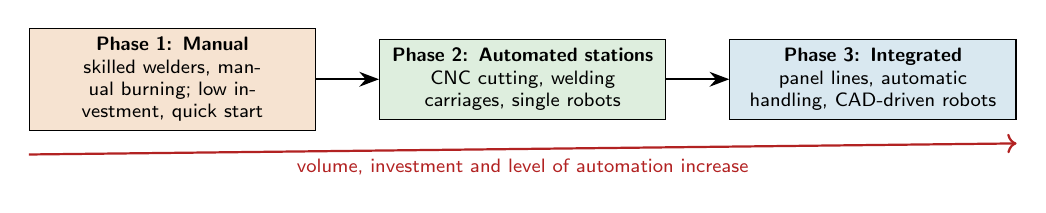
\begin{tikzpicture}[every node/.style={font=\scriptsize}, node distance=0.8cm]
					\node[process, fill=cOrange!18, text width=3.4cm] (p1) {\textbf{Phase 1: Manual}\\ skilled welders, manual burning; low investment, quick start};
					\node[process, right=of p1, fill=cGreen!15, text width=3.4cm] (p2) {\textbf{Phase 2: Automated stations}\\ CNC cutting, welding carriages, single robots};
					\node[process, right=of p2, fill=cAccent!15, text width=3.4cm] (p3) {\textbf{Phase 3: Integrated}\\ panel lines, automatic handling, CAD-driven robots};
					\draw[flowarrow] (p1) -- (p2); \draw[flowarrow] (p2) -- (p3);
					\draw[->, thick, cRed] ($(p1.south west)+(0,-0.3)$) -- ($(p3.south east)+(0,-0.3)$) node[midway, below] {volume, investment and level of automation increase};
				\end{tikzpicture}
			\end{center}
			Automation is introduced in steps as demand and experience grow: each phase is proven before the next investment, reducing risk, and the same product-model data are reused at every phase.
		\end{answer}

		% -------------------------------------------------------------
		\item Draw a flowchart of the shipbuilding production process. Explain the hull block construction method, zone outfitting, and the levels of automation at different production stages. \qmarks{10}
		\begin{answer}
			\textbf{(a) Production process}
			\begin{center}
				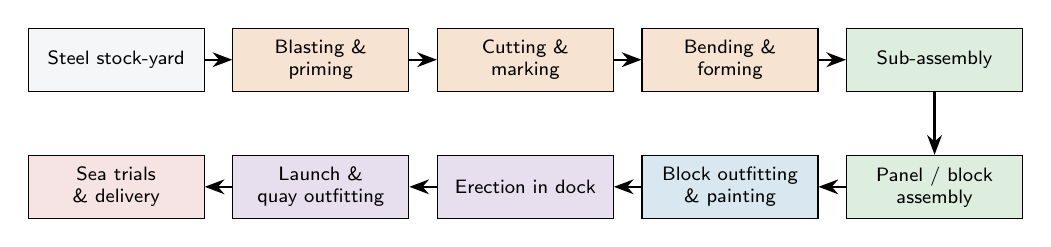
\begin{tikzpicture}[every node/.style={font=\scriptsize}, node distance=0.35cm,
					st/.style={process, minimum width=2.0cm, text width=2.0cm, minimum height=0.8cm}]
					\node[st, fill=cGrayBg] (s1) {Steel stock-yard};
					\node[st, right=of s1, fill=cOrange!18] (s2) {Blasting \& priming};
					\node[st, right=of s2, fill=cOrange!18] (s3) {Cutting \& marking};
					\node[st, right=of s3, fill=cOrange!18] (s4) {Bending \& forming};
					\node[st, right=of s4, fill=cGreen!15] (s5) {Sub-assembly};
					\node[st, below=0.8cm of s5, fill=cGreen!15] (s6) {Panel / block assembly};
					\node[st, left=of s6, fill=cAccent!15] (s7) {Block outfitting \& painting};
					\node[st, left=of s7, fill=cPurple!15] (s8) {Erection in dock};
					\node[st, left=of s8, fill=cPurple!15] (s9) {Launch \& quay outfitting};
					\node[st, left=of s9, fill=cRed!12] (s10) {Sea trials \& delivery};
					\draw[flowarrow] (s1) -- (s2); \draw[flowarrow] (s2) -- (s3); \draw[flowarrow] (s3) -- (s4); \draw[flowarrow] (s4) -- (s5);
					\draw[flowarrow] (s5) -- (s6); \draw[flowarrow] (s6) -- (s7); \draw[flowarrow] (s7) -- (s8); \draw[flowarrow] (s8) -- (s9); \draw[flowarrow] (s9) -- (s10);
				\end{tikzpicture}
			\end{center}

			\textbf{(b) Hull block construction method (HBCM)}: the hull is divided into \textbf{blocks} (50--900 t) built in parallel in covered workshops from parts, sub-assemblies and panels, then lifted by gantry cranes and \textbf{erected} in the dock. Benefits: parallel work, better access and working positions (down-hand welding), shorter dock time.

			\textbf{(c) Zone outfitting and zone painting}: pipes, cable trays, equipment foundations and machinery are fitted, and blocks are painted, \textbf{before} erection (on-block / on-unit outfitting). Work is done in the open, easy-to-reach block rather than in the finished ship, saving time and cost.

			\textbf{(d) Levels of automation by stage} (indicative)
			\begin{center}
				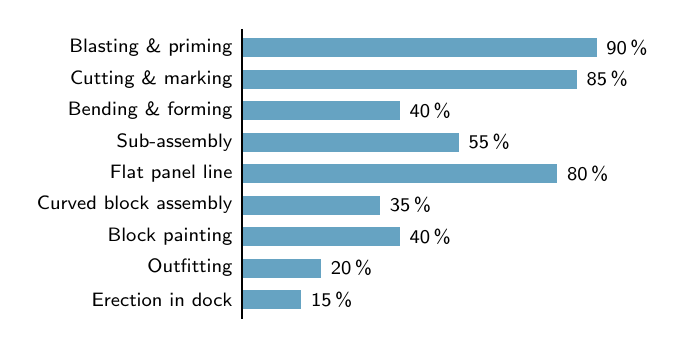
\begin{tikzpicture}[font=\scriptsize, x=0.05cm, y=0.4cm]
					\foreach \n/\v/\l in {0/90/{Blasting \& priming}, 1/85/{Cutting \& marking}, 2/40/{Bending \& forming}, 3/55/{Sub-assembly}, 4/80/{Flat panel line}, 5/35/{Curved block assembly}, 6/40/{Block painting}, 7/20/{Outfitting}, 8/15/{Erection in dock}} {
						\pgfmathsetmacro{\yy}{-\n}
						\node[left] at (0,\yy) {\l};
						\fill[cAccent!60] (0,\yy-0.3) rectangle (\v,\yy+0.3);
						\node[right] at (\v,\yy) {\v\,\%};
					}
					\draw[thick] (0,0.6) -- (0,-8.6);
				\end{tikzpicture}
			\end{center}
			Automation is \textbf{highest} where work is flat, straight and repetitive (plate lines, cutting, flat panels) and \textbf{lowest} where work is three-dimensional, confined or unique (curved blocks, outfitting, erection). Levels range from manual $\rightarrow$ mechanised (welding tractor) $\rightarrow$ semi-automatic (portable robot) $\rightarrow$ automatic (gantry robots) $\rightarrow$ integrated (CAD-driven, MES-controlled).
		\end{answer}

		% -------------------------------------------------------------
		\item Explain the use of robots in shipyard welding with a neat diagram of an automatic panel line and a flowchart of the portable welding-robot cycle. Show, with an example, how robots improve productivity. Briefly mention robots for blasting, painting and heavy lifting. \qmarks{10}
		\begin{answer}
			\textbf{(a) Automatic panel line}
			\begin{center}
				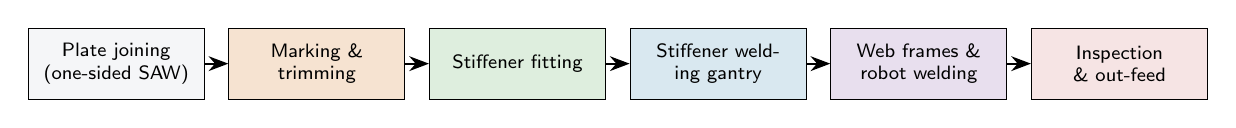
\begin{tikzpicture}[every node/.style={font=\scriptsize}, node distance=0.3cm,
					st/.style={process, minimum width=2.0cm, text width=2.0cm, minimum height=0.9cm}]
					\node[st, fill=cGrayBg] (a) {Plate joining (one-sided SAW)};
					\node[st, right=of a, fill=cOrange!18] (b) {Marking \& trimming};
					\node[st, right=of b, fill=cGreen!15] (c) {Stiffener fitting};
					\node[st, right=of c, fill=cAccent!15] (d) {Stiffener welding gantry};
					\node[st, right=of d, fill=cPurple!15] (e) {Web frames \& robot welding};
					\node[st, right=of e, fill=cRed!12] (f) {Inspection \& out-feed};
					\draw[flowarrow] (a) -- (b); \draw[flowarrow] (b) -- (c); \draw[flowarrow] (c) -- (d); \draw[flowarrow] (d) -- (e); \draw[flowarrow] (e) -- (f);
				\end{tikzpicture}
			\end{center}
			Flat panels move on roller conveyors from station to station (product layout). Multi-head gantry robots weld stiffeners on both sides at once, reducing distortion; weld paths come from the 3-D model (\textbf{off-line programming}).

			\noindent\begin{minipage}[t]{0.40\linewidth}
				\textbf{(b) Portable robot cycle}
				\begin{center}
					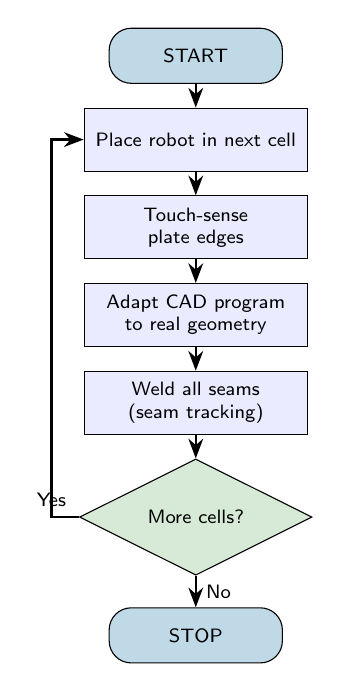
\begin{tikzpicture}[font=\scriptsize, node distance=0.3cm]
						\node[startstop] (st) {START};
						\node[process, below=of st] (p) {Place robot in next cell};
						\node[process, below=of p] (s) {Touch-sense plate edges};
						\node[process, below=of s] (a) {Adapt CAD program to real geometry};
						\node[process, below=of a] (w) {Weld all seams (seam tracking)};
						\node[decision, below=of w] (d) {More cells?};
						\node[startstop, below=0.4cm of d] (en) {STOP};
						\draw[flowarrow] (st) -- (p); \draw[flowarrow] (p) -- (s); \draw[flowarrow] (s) -- (a); \draw[flowarrow] (a) -- (w); \draw[flowarrow] (w) -- (d);
						\draw[flowarrow] (d) -- node[right] {No} (en);
						\draw[flowarrow] (d.west) -- ++(-0.35,0) node[above] {Yes} |- (p.west);
					\end{tikzpicture}
				\end{center}
			\end{minipage}\hfill
			\begin{minipage}[t]{0.57\linewidth}
				\textbf{Explanation}: small portable robots are lifted by crane into the \textbf{double-bottom cells}. Touch sensing finds the real plate positions, the CAD-generated program is corrected, and all fillet welds are made with arc seam tracking. Weld data are logged for class-society records.

				\medskip
				\textbf{(c) Productivity example}: 200 m of fillet weld, $t = L/(v\,f)$.
				\begin{itemize}[itemsep=1pt]
					\item Manual ($v = 0.3$ m/min, $f = 30\,\%$):\\
					$t = 200/(0.3\times0.3) = 2222$ min $\approx \mathbf{37.0\ h}$
					\item Robot ($v = 0.5$ m/min, $f = 80\,\%$):\\
					$t = 200/(0.5\times0.8) = 500$ min $\approx \mathbf{8.3\ h}$
					\item Time saved $\approx$ \textbf{77.5\,\%} --- mainly from the higher arc-on time.
				\end{itemize}
			\end{minipage}

			\medskip
			\textbf{(d) Other robots}
			\begin{itemize}[itemsep=1pt]
				\item \textbf{Blasting \& painting}: magnetic crawlers with grit or UHP water-jet heads (dust vacuumed back); boom/gantry painting robots keep a constant stand-off, angle and speed, giving uniform DFT and higher transfer efficiency (e.g.\ 85\,\% vs 60\,\%), saving about 29\,\% paint.
				\item \textbf{Heavy lifting}: Goliath gantry cranes with synchronised hoists and anti-sway control for block erection and turn-over; SPMTs with computer-controlled steering and hydraulic load levelling move blocks of several hundred tonnes.
			\end{itemize}
		\end{answer}

	\end{enumerate}

\end{document}
